\chapter{Implementation}\label{ch:implementation}

This chapter describes how the theory discussed in chapter \ref{ch:theory} has been implemented in our solution. We have divided the chapter into a overall section about the ARQ protocol and then sections per node, that is base station, the relay nodes and the runner node. For better readability, code snippets of the actual implementation has been turned into pseudo code. To view the nesC code please see the appendix.

\subsection{Generic ARQ implementation}\label{sc:overall}

The ARQ stop-and-wait method has been implemented on all nodes in the system. Figure \ref{fig:tohopornotarqsequence} is a sequence diagram of the  protocol implementation and shows how data requests are initiated by the base station and forwarded either directly to the runner (left side) or via a relay station (right side). Adding to this is the parity bit calculations to verify the integrity of received frames. This is conduced when a frame is received in either base station or one of the other nodes.

\begin{figure}[h]
	\centering
	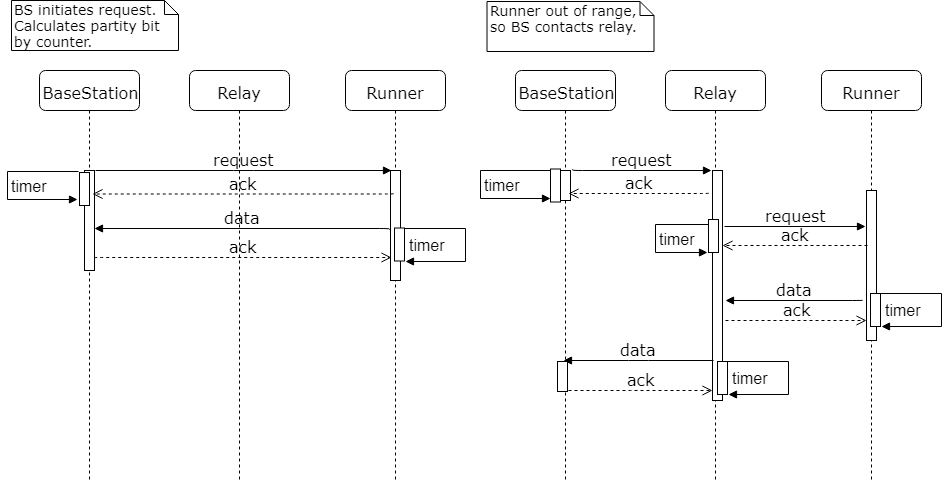
\includegraphics[width=1\linewidth]{implementation/overall/toHopOrNotArqSequence}
	\caption{The flow of data and acknowledgment messages between the nodes.}
	\label{fig:tohopornotarqsequence}
\end{figure}

\noindent The basics of the communications between the nodes are as follows: \\ \newline
1. The base station requests data at a certain time interval defined by a timer. When the timer runs out, it decides whether is should send the request directly or via one of the relays by using our protocol. To the request is attached a counter ($n = 0, 1, 2, 3$ -> $n$) and a sequence number (0 or 1) used by the receiver to verify the frame. When the radio is ready to transmit, it is forwarded to a specific node and the ARQ timer starts. It it now the responsibility of the receiving node to carry on the request. The receiver will send back a ACK frame to the base station if validation succeeded.\\ \newline
2. If the request reached the runner first, it will use the attached counter to calculate a new parity bit and compare this to the one in the request. If they match, it sends back an ACK followed by a data message containing the current heart rate of the athlete. A counter and a sequence number is attached to this as well.\\ \newline
3. The base station receives the data message, checks the parity bit, and saves it. It has now successfully obtained the heart rate.\\ \newline
4. If the base station decide to relay the request, the same procedure applies for the relay nodes. It is now the job of the relay to acknowledge the request, communicate with the runner using ARQ, obtain the data and send it back to the base station.\\ \newline
\noindent With ARQ and parity bit checking we archive a simple but reliable data-link connection between nodes and a way to discard damaged frames. One particular area of concern was the configuration of the timers, as they have to be consistent throughout the network. Obviously when relaying, the base station must take into account the turnaround time and possible retransmissions of the relay and the runner node before sending a new one. The base station timer ($Ba_t$) must be larger than the relay's ($Re_t$) and the runner's ($Ru_t$) combined, so $Ba_t$ > $Re_t$ + $Ru_t$ for the protocol to work correctly.

\section{Base station}\label{sc:basestation}

The base station is the master node in our setup. It is responsible for three import tasks: Initiating data requests, decide if the runner is out of range and keep track of past events. Figure \ref{fig:tohopornotarqsequence} shows the overall flow of data, but we shall examine the more detailed parts here.

\noindent The main control loop is started by a timer every $s$ second. It asserts if the runner is deemed out of range by calling a function and uses the feedback (either true or false) to increase an error counter that is used to change destination node. In other words, when a certain number of errors have occurred on the current link, we change request destination (from directly to relaying or vice versa). Listing \ref{lst:basestation1} is an example.
\noindent
\begin{minipage}[t]{0.95\linewidth}
	\begin{lstlisting}[language=Python, numbers=none, caption=XXX, label={lst:basestation1}]
Timer0.fired() {
	if out of range and link is direct {
		if the error count is below max
			use_next_destination
		else
			increase_error_count
	}
	if link is direct
		send_a_message_direct
	if link is relay to node north
		send_a_message_to_north
	if link is relay to node south
		send_a-message_to_south
}
	\end{lstlisting}
\end{minipage}

\noindent Next is how the base station determines if the runner is out range. When new replies are received directly from the runner (it starts in range) we save the RSSI\footnote{RSSI is a scalar register value on the CC2420 radio calculated from the RF input power in dBm.} value in a FIFO(First In First Out) queue with a length of 10. In such a queue, new data is inserted at back and taken out from the front. This means that the latest RSSI value of the runner is the back entry, with $n=0,1,2 ... 8$ being previous positions. Our algorithm takes a mean of these and multiplies it with a weighted score. If the latest position is lower than the mean, it is added to the weighted mean of the previous positions. If it is greater the average is then subtracted from it. The result constitutes a new estimated position of the runner. Listing \ref{lst:basestation2} is an example.

\noindent
\begin{minipage}[t]{0.95\linewidth}
\begin{lstlisting}[language=Python, numbers=none, caption=XXX, label={lst:basestation2}]
bool isOutOfRange {
	if current size of queue is not max
		return
	for(i = 0; i < queue_size; i++)
		previousPos += queue_part[i]
		
	lastPos = queue_back_entry
	mean = previousPos/queue_size
	
	if lastPos is less than mean
		newPos = (lastPos*1)+(mean*0.1);
	else
		newPos = (lastPos*1)-(mean*0.1);
	
	if(newPos is larger than threshold)
		return true;
	return false;
}
\end{lstlisting}
\end{minipage}

\noindent The weights used can be changed to put more empathize on the previous positions or more on the latest. Resulting on it acting more or less fast on new network conditions newest received packet.

\subsection{Relay}\label{sc:relay}
The Relay nodes in this setup are slaves to the base station. Their functionality is to relay messages to the Runner node, where the base station node is out of reach. Because of this the Relay node listens to the network and in case of being spoken to, will reply with an acknowledge and further send data to the Runner node. In case that the Relay node is not able to get in contact with the Runner node after three times, it sends an error message to the Base station.

\begin{minipage}[t]{0.95\linewidth}
	\begin{lstlisting}[caption=Receive message event of Relay., label={lst:relay1}]
event message_t * Receive.receive(message_t *msg, void *payload, uint8_t len){
	if (len == sizeof(requestMessage)) {
		requestMessage* reqmsg = (requestMessage*) payload;
		
		if (reqmsg->relayNodeid == TOS_NODE_ID) {
			// Send Acknowledge
			sendAcknowledge(reqmsg);
			
			if (reqmsg->data == 0) {	
				requestFromBase = *reqmsg;
				call Timer0.startPeriodic(TIMER0_PERIOD_MILLI);		
			}
			else {
				requestFromRunner = *reqmsg;
				call Timer1.startPeriodic(TIMER1_PERIOD_MILLI);
			}
		}
	}
	\end{lstlisting}
\end{minipage}

\noindent On listing \ref{lst:relay1} the main functionality of the Relay nodes can be seen. The Relay nodes are always in need of commands to them before sending a command themselves, they won't work on their own and therefore relies on requests from the Base station and answers from the Runner.

\subsection{Runner}\label{sc:runner}

The runner node's task in our WSN is to respond to data request messages sent from the base station or the relay nodes, as seen in the sequence digram in figure \ref{fig:tohopornotarqsequence}. The node contains various settings that can configured as constants, so they are easy to change eg. the transmit channel and the radiation power of the antenna. When it receives a packet it will check that the packet was intended for the runner and if so it will send an ACK to the requester and get ready to send the data as a subsequent reply.

\begin{minipage}[t]{0.95\linewidth}
\begin{lstlisting}[label={lst:runner1}, caption={Runner receives requests and responds.}]
Receive.receive(Message pkt){
	if pkt is requestMessage {
		if request is for runner {
			send_Acknowledgement
			Timer_sendDataTorequester
		}
	} 
}
\end{lstlisting}
\end{minipage}

\noindent The data contains the heart rate of the runner and in this scenario we just return a constant value. When sending data to the requesting node, it will start a timer and if it does not receive an ACK within a fixed time, it will resend the message three times followed by giving up on that reply.

\begin{minipage}[t]{0.95\linewidth}
\begin{lstlisting}[label={lst:runner2}, caption={Runner sends data packet with runner's heart rate.}]
sendData() {
	if If is not AntenaBusy {
		responsePacket_pulseData add runner_heart_beat
		if AMSend_send(responsepkt) is SUCCESS {
			AntenaBusy to TRUE
			resendCounter++
		}
	}
	if resendCounter is bigger then and equal to TRIES_TO_RESEND {
		resendCounter = 0
	}
}
\end{lstlisting}
\end{minipage}

\section{Energy Lab}\label{sc:energylab}

To test the 